
\documentclass[11pt,a4paper,hidelinks,fleqn]{article}            % Article 12pt font for a4 paper while hiding links
\usepackage[margin=1in]{geometry}                          % Required to adjust margins
../styleAndCommands.tex
\date{}
\begin{document}

\subsection*{Question 1 [20 marks]}

\paragraph{a)} For the function $f(x) = 4x^3 + 4 x - 5, ~x\in[0, 10]$,
describe an algorithm in pseudo code for finding the root of $f(x) = 0$ using the Regula Falsi method.

\paragraph{b)} Calculate the first two iterations of the Regula Falsi method used in a).

\subsection*{Question 2 [20 marks]} 

The function $f(x)$ is four times continuously differentiable ($C^4$).
Given 5 sample points of the function $[f(x_0-h), f(x_0-\frac{h}{2}), f(x_0), f(x_0+\frac{h}{2}), f(x_0+h)]$,
describe the algorithm to approximate $f'(x_0)$ through:

\paragraph{a)} combining the taylor expansions at the four points $f(x_0-h), f(x_0-\frac{h}{2}), f(x_0+\frac{h}{2}), f(x_0+h)$
with the goal to achieve the highest possible order of accuracy;

\paragraph{b)} Richardson extrapolation with $g(h)$ and $g(\frac h2)$, where $g(h)$ is the central difference at $x_0$ with step size $h$; 

\paragraph{c)} constructing the polynomial of order 4, $p(x) = \sum_{i=0}^4 a_i x^i$, passing by the 5 given points and taking the derivative of the polynomial at $x_0$.



\subsection*{Question 3 [20 marks]}
Consider the following one step binomial tree model of the stock price process:
\begin{figure*}[h]
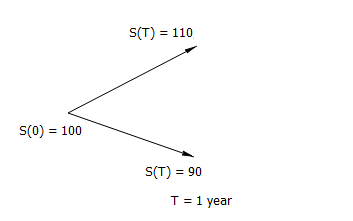
\includegraphics[scale=0.9]{./4}
\end{figure*}

a) Assume interest rate is $0\%$, compute the price of a call option struck at 100 at maturity 1 year using the method of the replicating portfolio.

b) Assume interest rate is $5\%$, compute the price of a call option struck at 100 at maturity 1 year using the method of the replicating portfolio.


\subsection*{Question 4 [20 marks]} 
Consider the numerical integration of 
\begin{align*}
\int_0^{2} f(x) dx, ~~\text{where~} f(x) = \frac{1}{2} e^{-\frac12x^2}
\end{align*}

\paragraph{a)} Evaluate the integral by mid-point quadrature with 4 equally spaced intervals. 

\paragraph{b)} Describe in pseudo code the algorithm to evaluate the integral using Monte-Carlo simulation.
 

\paragraph{c)} You would like to use $g(x)$, the second order Taylor 
expansion of $f(x)$ at $x=0$, as control variate. 
Assume you know already the variance of $g(x)$ and covariance of $[f, g]$.
Write down the expression of $g(x)$, 
and explain what change you need to make in the Monte-Carlo integration algorithm in b) to use $g(x)$ as control variate.


\subsection*{Question 5 [20 marks]}
Consider the process $X_t$
\begin{align*}
dX_t = \sigma dW_t
\end{align*}
where $W_t$ is a standard Wiener process and $\sigma$ is the constant volatility.
Denote $V_t$ the price of a derivative on the process.

\paragraph{a)} Derive the partial differential equation satisfied by $V(x, t)$.

\paragraph{b)} Assume the risk-free interest rate is 0,
discretize the partial differential equation using finite difference in both time and x axis with explicit Euler scheme,
write down the equation that computes $V(x, t_i)$ from the time slice $t_{i+1}$.

\paragraph{c)} Suppose that the derivative's price at $t_{i+1}$ is of the form shown in the below chart,
i.e., $V(x, t_{i+1})$ is known, 
sketch the rough shape of $V(x, t_{i})$ on top of the plot and explain the rationale.
\begin{figure*}[h]
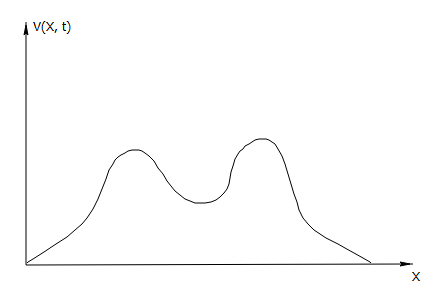
\includegraphics[scale=0.9]{./6c} \\
\vspace{1cm}
\textbf{*END OF PAPER*}
\end{figure*}



\end{document}
